\documentclass[11pt, a4paper]{article}
\usepackage[utf8]{inputenc}
\usepackage[norsk]{babel} % Setter dokumentet til norsk
\usepackage{amsmath}      % Nødvendig for ligningene (align)
\usepackage{amssymb}      % Nødvendig for matematiske symboler som \min
\usepackage{geometry}     % Setter normale marginer på arket
\geometry{margin=1in}
\usepackage{tikz}
\usetikzlibrary{shapes,arrows,positioning}
\begin{document}

\section*{Komplett utledning av SIMC PI-regler}

\subsection*{1. Utledning av lukket sløyfe}
\begin{figure}[htbp]
\centering
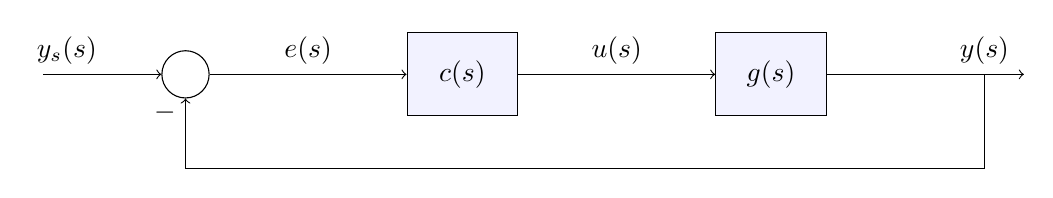
\begin{tikzpicture}[
    node distance=2.5cm,
    block/.style={draw, rectangle, minimum height=3em, minimum width=4em, fill=blue!5},
    sum/.style={draw, circle, node distance=1.5cm, inner sep=0pt, minimum size=6mm},
    input/.style={coordinate},
    output/.style={coordinate}
]

    % Plasserer nodene i diagrammet (fra venstre mot høyre)
    \node [input, name=input] {};
    \node [sum, right=of input] (sum) {};
    \node [block, right=of sum] (regulator) {$c(s)$};
    \node [block, right=of regulator] (process) {$g(s)$};
    \node [output, right=of process, node distance=2cm] (output) {};

    % Tegner linjene og pilene mellom nodene
    \draw [draw,->] (input) -- node[pos=0.2, above] {$y_s(s)$} (sum);
    \draw [->] (sum) -- node[above] {$e(s)$} (regulator);
    \draw [->] (regulator) -- node[above] {$u(s)$} (process);
    \draw [->] (process) -- node [name=y, pos=0.8, above] {$y(s)$} (output);
    
    % Tegner tilbakekoblingssløyfen (feedback)
    \draw [->] (y) |- ++(0,-1.5) -| node[pos=0.9, left] {$-$} (sum);

\end{tikzpicture}
\caption{Blokkdiagram for det lukkede reguleringssystemet med negativ tilbakekobling.}
\label{fig:blokkdiagram}
\end{figure}

Vi tar utgangspunkt i en standard reguleringssløyfe med negativ tilbakekobling:
\begin{align}
    e(s) &= y_s(s) - y(s) \\
    u(s) &= c(s) \cdot e(s) \\
    y(s) &= g(s) \cdot u(s)
\end{align}
Substitusjon av ligning (1) og (2) inn i (3) gir:
\begin{equation}
    y(s) = g(s)c(s)\left[ y_s(s) - y(s) \right]
\end{equation}
Multipliserer ut parentesen og samler $y(s)$ på venstre side:
\begin{equation}
    y(s) + c(s)g(s)y(s) = c(s)g(s)y_s(s)
\end{equation}
Faktoriserer ut $y(s)$ og løser for overføringsfunksjonen til det lukkede systemet:
\begin{equation}
    \frac{y(s)}{y_s(s)} = \frac{c(s)g(s)}{1 + c(s)g(s)}
\end{equation}

\subsection*{2. SIMC-utledning for $K_c$ og $\tau_I$}
Vi betrakter en førsteordens prosess med tidsforsinkelse (FOPTF):
\begin{equation}
    g(s) = \frac{k}{\tau s + 1} e^{-\theta s}
\end{equation}
Skogestad spesifiserer en ønsket førsteordens lukket sløyfe-respons:
\begin{equation}
    \frac{y(s)}{y_s(s)} = \frac{1}{\tau_c s + 1} e^{-\theta s}
\end{equation}
Vi løser ligning (6) med hensyn på regulatoren $c(s)$ gjennom direkte syntese:
\begin{equation}
    c(s) = \frac{1}{g(s)} \frac{\frac{y(s)}{y_s(s)}}{1 - \frac{y(s)}{y_s(s)}}
\end{equation}
Setter inn den ønskede responsen fra (8):
\begin{equation}
    c(s) = \frac{1}{g(s)} \frac{e^{-\theta s}}{(\tau_c s + 1) - e^{-\theta s}}
\end{equation}
Vi benytter en førsteordens Taylor-approksimasjon for tidsforsinkelsen i nevneren, $e^{-\theta s} \approx 1 - \theta s$:
\begin{equation}
    (\tau_c s + 1) - e^{-\theta s} \approx \tau_c s + 1 - (1 - \theta s) = (\tau_c + \theta)s
\end{equation}
Innsetting av prosessmodellen (7) og approksimasjonen (11) inn i (10) gir:
\begin{equation}
    c(s) = \frac{\tau s + 1}{k\cdot e^{-\theta s}} \cdot \frac{e^{-\theta s}}{(\tau_c + \theta)s} = \frac{\tau s + 1}{k(\tau_c + \theta)s}
\end{equation}
Dette omformes til en standard PI-regulatorform:
\begin{equation}
    c(s) = \frac{\tau}{k\cdot(\tau_c + \theta)} \left( 1 + \frac{1}{\tau s} \right)
\end{equation}
Ved å sammenligne (13) med den ideelle PI-regulatoren $c(s) = K_c \left( 1 + \frac{1}{\tau_I s} \right)$, identifiserer vi parametrene:
\begin{equation}
    K_c = \frac{\tau}{k\cdot(\tau_c + \theta)}
\end{equation}
\begin{equation}
    \tau_I = \tau
\end{equation}
For å sikre rask forstyrrelsesavvisning for prosesser med stor tidskonstant, innfører Skogestad den modifiserte integraltiden:
\begin{equation}
    \tau_I = \min(\tau, \, 4(\tau_c + \theta))
\end{equation}

\end{document}
